\chapter{Problem setup}
\section{Overview of the Flexible Robotic Arm Model}
% - Define all parameters using the provided parameter sets.

This work addresses the optimal control of a planar two-link robotic manipulator characterized by its underactuated nature. The system dynamics evolve in a two-dimensional plane and consist of two rigid links connected by revolute joints, with actuation provided only at the first joint through an applied torque $u$.

\begin{figure}[htb]
    \centering
    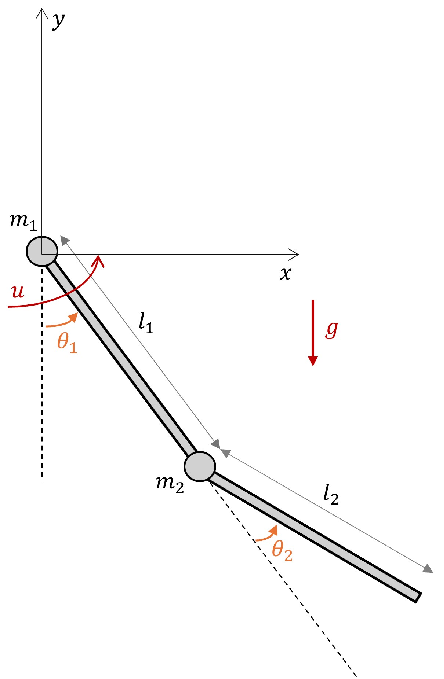
\includegraphics[width=0.35\linewidth]{img/0-task0/system.pdf}
    \caption{Model of the flexible arm.} %do not forget to add \cite{} inside caption if it is noy your picture
    \label{fig:flexible-arm}
\end{figure}

The system state is defined as $\mathbf{x} = [\dot{\theta}_1, \dot{\theta}_2, \theta_1, \theta_2]^\top \in \mathbb{R}^4$, where $\theta_1$ denotes the angle of the first link with respect to the vertical axis, $\theta_2$ represents the relative angle between the two links, and $\dot{\theta}_1$, $\dot{\theta}_2$ are their respective angular velocities. The control input $u \in \mathbb{R}$ acts as a torque at the first joint only, making the system underactuated.

The equations of motion are described by:
\begin{equation}
\mathbf{M}(\theta_1, \theta_2)\begin{bmatrix}\ddot{\theta}_1\\ \ddot{\theta}_2\end{bmatrix} + 
\mathbf{C}(\theta_1, \theta_2, \dot{\theta}_1, \dot{\theta}_2) + 
\mathbf{F}\begin{bmatrix}\dot{\theta}_1\\ \dot{\theta}_2\end{bmatrix} + 
\mathbf{G}(\theta_1, \theta_2) = \begin{bmatrix}u\\ 0\end{bmatrix}
\label{eq:dynamics}
\end{equation}

where $\mathbf{M}(\theta_1, \theta_2) \in \mathbb{R}^{2\times2}$ is the inertia matrix, $\mathbf{C}(\theta_1, \theta_2, \dot{\theta}_1, \dot{\theta}_2) \in \mathbb{R}^2$ accounts for Coriolis and centrifugal forces, $\mathbf{G}(\theta_1, \theta_2) \in \mathbb{R}^2$ describes gravitational effects, and $\mathbf{F} \in \mathbb{R}^{2\times2}$ represents viscous friction through a diagonal matrix. The dynamics parameters used in this analysis are presented in Table~\ref{tab:parameters}.

\begin{table}[htbp]
\centering
\caption{System Dynamics Parameters}
\label{tab:parameters}
\begin{tabular}{clc}
\hline
Parameter & Value \\
\hline
$M_1$ & 2.0 [kg] \\
$M_2$ & 2.0 [kg] \\
$L_1$ & 1.5 [m] \\
$L_2$ & 1.5 [m] \\
$R_1$ & 0.75 [m] \\
$R_2$ & 0.75 [m] \\
$I_1$ & 1.5 [kg$\cdot$m$^2$] \\
$I_2$ & 1.5 [kg$\cdot$m$^2$] \\
$g$ & 9.81 [m/s$^2$] \\
$F_1$ & 0.1 [N$\cdot$m$\cdot$s/rad] \\
$F_2$ & 0.1 [N$\cdot$m$\cdot$s/rad] \\
\hline
\end{tabular}
\end{table}

\section{Discretization of Dynamics}

\subsection{Discretization Using Euler Method}

The continuous-time dynamics described in Equation~\ref{eq:dynamics} are discretized using the Euler method for implementation in a digital control system. The time derivative is approximated as:
\[
\dot{x} \approx \frac{x_{k+1} - x_k}{\Delta t}
\]
where \(\Delta t\) is the sampling time. Rearranging this yields the discrete-time update:
\[
x_{k+1} = x_k + \Delta t \cdot dx
\]
where \(dx\) is computed as:
\[
dx = A x_k + B u_k + c
\]

\begin{itemize}
    \item \(A\) is the system matrix derived from the inertia, damping, and coupling effects, with terms dependent only on $\mathbf{x}$,
    \item \(B\) is the input matrix, with terms dependent only on $\mathbf{u}$,
    \item \(c\) encapsulates non-linear effects such as Coriolis, centrifugal, and gravitational forces.
\end{itemize}

\noindent The explicit equation of $dx$ is the following:
\begin{equation}
\begin{bmatrix}
    \ddot \theta_1 \\
    \ddot \theta_2 \\
    \dot \theta_1 \\
    \dot \theta_2 \\
\end{bmatrix}
=
\begin{bmatrix}
    -\mathbf{M}^{-1} \mathbf{F} & 0_{2 \times 2} \\
    I_{2 \times 2} & 0_{2 \times 2}
\end{bmatrix}
\begin{bmatrix}
    \dot \theta_1 \\
    \dot \theta_2 \\
    \theta_1 \\
    \theta_2
\end{bmatrix}
+
\begin{bmatrix}
    \mathbf{M}^{-1} & 0_{2 \times 2} \\
    0_{2 \times 2} & 0_{2 \times 2}
\end{bmatrix}
\begin{bmatrix}
    \tau_1 \\
    \tau_2 \\
    0 \\
    0
\end{bmatrix}
+
\begin{bmatrix}
    -\mathbf{M}^{-1} (\mathbf{C} + \mathbf{G}) \\
    0_{2 \times 1}
\end{bmatrix}
\label{eq:state-update}
\end{equation}

Since the system is underactuated, $\tau_2$ is always zero.
